\documentclass[12pt,a4paper,fleqn]{article}
\usepackage{rmpackages}																% usual packages
\usepackage{rmtemplate}																% graphic charter
\usepackage{rmexocptce}																% for DS with cptce eval

\cfoot{} 													% if no page number is needed
%\renewcommand\arraystretch{1.5}		% stretch table line height

\begin{document}

\begin{header}
Les défis confinés -- Épisode 9
\end{header}

\section*{L'oeil}

L'oeil est un instrument optique remarquable.
Il est capable de s'adapter pour observer des objets très éloignés, tout comme des objets très proches.

Regarder la vidéo \href{https://youtu.be/4qc5MMKZIIw}{https://youtu.be/4qc5MMKZIIw}.

\begin{enumerate}
\item Associer à chacun des éléments de l'œil réel l'élément correspondant dans le modèle réduit de l'œil.
\begin{center}
\begin{tabular}{rcccl}
Rétine & $\bullet$ & \hspace{50pt} & $\bullet$ & Lentille \\
Cristallin et autres milieux transparents & $\bullet$ & \hspace{50pt} & $\bullet$ & Diaphragme \\
Iris & $\bullet$ & \hspace{50pt} & $\bullet$ & Écran
\end{tabular}
\end{center}

\item À quelle condition l'image d'un objet perçue par l'œil est-elle nette ?

\item Reproduire les deux schémas ci-dessous.
Dans laquelle de ces deux situations l'image perçue par l'œil (schématisé par la lentille et l'écran) sera-t-elle nette ?
\end{enumerate}

\begin{multicols}{2}
\begin{center}
\newcommand{\width}{8}
\newcommand{\height}{3}
\newcommand{\step}{.25}
\begin{tikzpicture}
\foreach \y in {0,\step,...,\height} {
    \draw [gray_c] (0,\y) --++ (\width,0);
}
\foreach \x in {0,\step,...,\width} {
    \draw [gray_c] (\x,0) --++ (0, \height);
}

\pgfmathsetmacro\x{(\width)/2}
\pgfmathsetmacro\y{(\height)/2}
\coordinate (O) at (\x,\y);
\draw [->, >=stealth, thick] (0, \y) --++ (\width, 0);

\draw [<->, >=angle 60, ultra thick] (\x, 0) -- (\x, \height);
\draw (O) node [below left] {$O$};
\draw (O) ++ (-1.5, 0) node [below left] {$F$};
\draw (O) ++ (-1.5, 0) node {$|$};
\draw (O) ++ (1.5, 0) node [below left] {$F'$};
\draw (O) ++ (1.5, 0) node {$|$};

\draw [->, >=stealth, ultra thick, red] (O) ++ (-3, 0) node [below left] {$A$} --++ (0, 1) node [below left] {$B$};

\draw [ultra thick] (O) ++ (3, -\y) --++ (0,\height) node [below left] {écran};
\end{tikzpicture}

\begin{tikzpicture}
\foreach \y in {0,\step,...,\height} {
    \draw [gray_c] (0,\y) --++ (\width,0);
}
\foreach \x in {0,\step,...,\width} {
    \draw [gray_c] (\x,0) --++ (0, \height);
}

\pgfmathsetmacro\x{(\width)/2}
\pgfmathsetmacro\y{(\height)/2}
\coordinate (O) at (\x,\y);
\draw [->, >=stealth, thick] (0, \y) --++ (\width, 0);

\draw [<->, >=angle 60, ultra thick] (\x, 0) -- (\x, \height);
\draw (O) node [below left] {$O$};
\draw (O) ++ (-1, 0) node [below left] {$F$};
\draw (O) ++ (-1, 0) node {$|$};
\draw (O) ++ (1, 0) node [below left] {$F'$};
\draw (O) ++ (1, 0) node {$|$};

\draw [->, >=stealth, ultra thick, red] (O) ++ (-3, 0) node [below left] {$A$} --++ (0, 1) node [below left] {$B$};

\draw [ultra thick] (O) ++ (3, -\y) --++ (0,\height) node [below left] {écran};
\end{tikzpicture}
\end{center}
\end{multicols}

\begin{enumerate}[resume]
\item Quelle propriété de la lentille a été modifiée ?

\item Comment s'appelle l'action réalisée par l'œil pour modifier ce paramètre ?

\item \textit{Bonus : Dans la situation où l'image n'est pas nette, où devrait-on placer l'objet pour que son image soit nette ?}
\end{enumerate}

\section*{Pour aller plus loin...}

Un épisode de C'est pas sorcier : \href{https://youtu.be/2va8DyKjw7s}{https://youtu.be/2va8DyKjw7s}.

\end{document}

\begin{multicols}{2}
\begin{center}
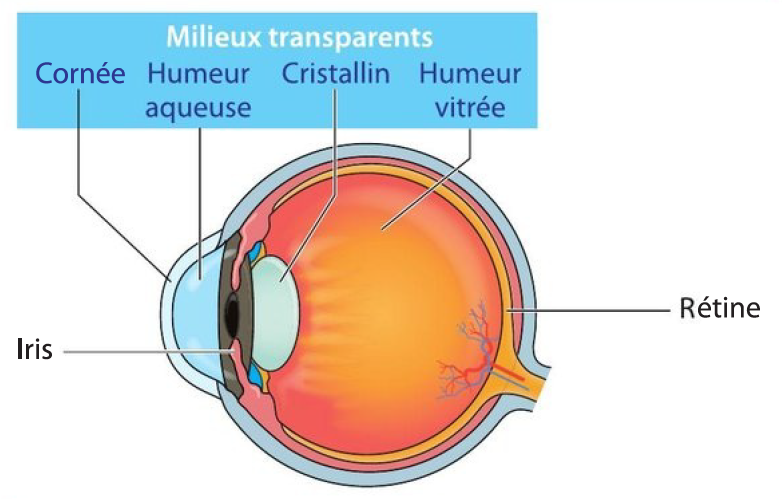
\includegraphics[width=\linewidth]{images/oeil_schema.png}
Schéma de l'œil réel

\columnbreak
\null\vfill
\begin{tikzpicture}
\coordinate (O) at (0,0);
\draw [->, >=stealth, thick] (-.25*\linewidth, 0) --++ (\linewidth, 0);
\draw [<->, >=angle 60, ultra thick, green_f] (0, -2) -- (0, 2);
\draw [ultra thick, green_f] (.7*\linewidth,-2) -- (.7*\linewidth,2);
\draw [ultra thick, green_f] (-.1*\linewidth,-2) -- (-.1*\linewidth,-1.25);
\draw [ultra thick, green_f] (-.1*\linewidth,2) -- (-.1*\linewidth,1.25);
\end{tikzpicture}
Modèle réduit de l'œil
\vfill{}
\end{center}
\end{multicols}

\begin{enumerate}[resume]
\item Reproduire le modèle réduit de l'œil
\end{enumerate}